\chapter{Product Specification}\hyperdef{part}{spec}{}\label{ch:spec}

\section{Conceptual Design}
\label{sec:conceptual_design}

The \ModelDesc has two overarching goals:
\begin{itemize}
\item Provide a generic framework for saving to and restoring from a checkpoint
file those resources that are opaque to the typical simulation engine.
\item Provide checkpointable and restorable replacements for
the STL container class templates.
\end{itemize}

This section provides insight into how the model achieves these goals.

\subsection{Key Concepts}\label{sec:key_concepts}
This section describes the key concepts that form the conceptual foundation of
the \ModelDesc.

\subsubsection{Checkpoint/Restart}\label{sec:key_checkpoint}
Checkpoint/restart addresses the issue of saving a description of a running
application in a manner that the application can later be restarted from
that saved description. Checkpoint/restart can be performed by the
operating system or by the application itself, and the checkpoint file can
be in text or binary form.

JEOD is primarily aimed at running in the Trick simulation environment, which
provides a text-based, application-side checkpoint/restart capability.
The basic Trick checkpoint/restart capability is, by design, incomplete.
Trick provides the ability to register functions as checkpoint or restart
jobs. A complete checkpoint/restart capability can be achieved by
augmenting Trick's basic checkpoint/restart capabilities with the right
combination of checkpoint and restart jobs.

This model does not provide the checkpoint/restart functions needed to make
a Trick checkpoint complete. What this model does provide are data
representations that simplify those checkpoint/restart functions in
the \SIMINTERFACE\ model.

\subsubsection{STL Containers}\label{sec:key_STL}
One of the key culprits that formerly made JEOD incapable of being
checkpoint/restart complete was its extensive use of STL containers.
Trick's data-driven checkpoint/restart mechanism does not jibe well
with the complex implementation of STL containers in most compilers.
The Trick project elected early on in the Trick 10 development process
to exclude STL containers from its data-driven checkpoint/restart approach.

The first step in making JEOD's use of the STL containers
checkpoint/restart-capable required providing functional equivalents of these
STL containers.
The model provides these function equivalents in the form of STL replacement
class templates. These replacements do not re-implement the STL containers.
They instead provide encapsulations of the containers. The interfaces to
those replacement templates is by design a near-duplicate of the public interfaces to the STL containers.

\subsubsection{Checkpointable/Restartable Objects}\label{sec:key_checkpointable}
The above STL replacements by themselves do nothing to solve the
checkpoint/restart problem. If anything, they exacerbate the problem by hiding
the encapsulated STL object from the simulation engine.

The approach taken within the model is to provide an abstract framework
for checkpoint and restart. Mixin class templates provided by the model
augment the basic STL replacement class templates with this checkpoint/restart
functionality. An added benefit of this scheme is that the same framework
can also be used to address other checkpoint/restart issues such as
checkpointing and restoring file descriptors.


\subsection{Model Architecture}
The \ModelDesc is implemented in the form of \Cplusplus classes and class
templates, described below.
\begin{description}
\item[\bf\code{JeodCheckpointable}] The base class for checkpointing and
  restarting data that are opaque to Trick,
  and presumably other simulation engines.
\item[\bf\code{SimpleCheckpointable}] A simplified version of
\code{JeodCheckpointable}.
\item[\bf\code{JeodSTLContainer}] A non-checkpointable replacement
  for STL containers in general.
\item[\bf\code{JeodAssociativeContainer}] A non-checkpointable replacement
  for STL associative containers.
\item[\bf\code{JeodSequenceContainer}] A non-checkpointable replacement
  for STL sequence containers.
\item[\bf\code{JeodList}] A non-checkpointable replacement for STL lists.
\item[\bf\code{JeodSet}] A non-checkpointable replacement for STL sets.
\item[\bf\code{JeodVector}] A non-checkpointable replacement for STL vectors.
\item[\bf\code{JeodContainer}] A mixin class that adds checkpoint/restart
  capabilities to a non-checkpointable JEOD STL container replacement.
\item[\bf\code{JeodObjectContainer}] A \code{JeodContainer}-derived class
  that addresses containers that contain object.
\item[\bf\code{JeodPointerContainer}] A \code{JeodContainer}-derived class
  that addresses containers that contain pointers.
\item[\bf\code{JeodPrimitiveContainer}] A \code{JeodContainer}-derived class
  that addresses containers that contain simple data.
\item[\bf\code{JeodPrimitiveSerializer}] Class used by
  \code{JeodPrimitiveContainer} to serialize/deserialize a simple piece of data.
\item[\bf\code{JeodObjectList}] A \code{Checkpointable} replacement
  for a list of objects.
\item[\bf\code{JeodObjectSet}] A \code{Checkpointable} replacement
  for a set of objects.
\item[\bf\code{JeodObjectVector}] A \code{Checkpointable} replacement
  for a vector of objects.
\item[\bf\code{JeodPointerList}] A \code{Checkpointable} replacement
  for a list of pointers.
\item[\bf\code{JeodPointerSet}] A \code{Checkpointable} replacement
  for a set of pointers.
\item[\bf\code{JeodPointerVector}] A \code{Checkpointable} replacement
  for a vector of pointers.
\item[\bf\code{JeodPrimitiveList}] A \code{Checkpointable} replacement
  for a list of primitives.
\item[\bf\code{JeodPrimitiveSet}] A \code{Checkpointable} replacement
  for a set of primitives.
\item[\bf\code{JeodPrimitiveVector}] A \code{Checkpointable} replacement
  for a vector of primitives.
\end{description}

\section{Key Algorithms}
\label{sec:algorithms}
The majority of the functions defined in the \ModelDesc are simple pass-through
functions to the encapsulated STL object. This section describes the
key algorithms within the model in the broader context of the
serialization and deserialization processes that form the basis of
text-based checkpoint and restart.

\subsection{Pointer Containers}
From the perspective of this model, containers of pointers are by far the
easiest to checkpoint and restart. The \SIMINTERFACE\ provides methods
to convert a pointer to a named representation of the pointed-to object and
to convert a named representation to a \code{void*} pointer. These methods
provide a natural serialization/deserialization mechanism for containers
of pointers.

\subsection{Object Containers}
Containers of objects are checkpointed by making a C-style array that is a
copy of the contained objects. The simulation engine is responsible for
checkpointing the contents of this array. The simulation engine is similarly
responsible for restoring the array on restart. With this copy,
the container itself is checkpointed and restarted by using the same
serialization/deserialization mechanism used for pointer containers.

\subsection{Primitive Containers}
Containers of primitives are checkpointed and restarted by using the
stream insertion and extraction operators for serialization and deserialization.
Special care is needed for strings, which can contain special characters, and floating point numbers, which have special
values to indicate the number is not-a-number (NaN) or infinity.
During serialization, special characters in strings are backslash-escaped
and  special numbers are serialized  as special-purpose strings.
The deserialization restores the special characters and special numbers. 

\section{Interactions}
\label{sec:interactions}

\subsection{JEOD Models Used by the \ModelDesc}
The \ModelDesc uses the following JEOD models:
\begin{itemize}
\item\hypermodelref{MEMORY}.
  The class template \code{JeodContainer} contains a pointer to
  a \MEMORY\ descriptor of the type of data in the container.
  The class template \code{JeodObjectContainer} uses the \MEMORY\ to
  allocate and destroy an array of objects whose contents
  are checkpointed and restored by the simulation engine.
\item\hypermodelref{SIMINTERFACE}.
  All \ModelDesc header files
  \code{\#include} the \SIMINTERFACE\ header file jeod\_class.hh.
  The class templates
  \code{JeodObjectContainer} and \code{JeodPointerContainer}
  use the \SIMINTERFACE\ to translate addresses to and from
  address specification strings.
\end{itemize}

\subsection{Use of the \ModelDesc in JEOD}
The following JEOD models use the \ModelDesc:
\begin{itemize}
\item\hypermodelref{MEMORY}.
  The \MEMORY\ provides the means by which JeodCheckpointable objects
  are registered with the \SIMINTERFACE\ for subsequent checkpoint/restart
  operations.
\item\hypermodelref{SIMINTERFACE}.
  The \SIMINTERFACE\ provides the mechanisms that checkpoint and restore
  JeodCheckpointable objects.
\item \hypermodelref{EPHEMERIDES} and \hypermodelref{DYNBODY}.
  The \EPHEMERIDES\ and \DYNBODY\ define subclasses of the SimpleCheckpointable
  class to restore opaque content defined by those models.
\item Several models.
  Many JEOD models use the STL container replacements provided
  by the \ModelDesc.
\end{itemize}

\subsubsection{\SIMINTERFACE}
\paragraph{Checkpoint.}
A JeodCheckpointable object is checkpointed by recording a series of triples,
object identifier, action, and value, that collectively provide the information
needed to later restore the contents of the object.

The following actions must be taken to checkpoint a JeodCheckpointable object:
\begin{enumerate}
\item If the string returned by object.get\_init\_name() is not empty,
the checkpoint agent must record a triple comprising
the object identifier,
the string returned by get\_init\_name(), and
the string returned by get\_init\_value().
\item Repeatedly record triples comprising
the object identifier,
the string returned by get\_item\_name(), and
the string returned by get\_item\_value().
This should be done as the body of a loop that iterates
over the object's checkpointable content.
\item If the string returned by object.get\_final\_name() is not empty,
the checkpoint agent must record a triple comprising
the object identifier,
the string returned by get\_final\_name(), and
the string returned by get\_final\_value().
\end{enumerate}
\begin{codeblock}
const std::string & init_action = object.get_init_name();
if (! init_action.empty()) {
   record (identifier, init_action, object.get_init_value());
}

for (object.start_checkpoint();
     !object.is_checkpoint_finished();
     object.advance_checkpoint()) {
   record (identifier, object.get_item_name(), object.get_item_value());
}

const std::string & final_action = object.get_final_name();
if (! final_action.empty()) {
   record (identifier, final_action, object.get_init_value());
}
\end{codeblock}

\paragraph{Restart.}
The JeodCheckpointable objects are restored to their checkpoint state by
transforming by parsing the checkpointed contents into
a set of identifier/action/value triples. For each triple,
the identifier is mapped to a pointer to a checkpointable object
and the object's \code{perform\_action} method is called with the
action and value supplied as arguments.

\clearpage
\section{Detailed Design}
\label{sec:detailed_design}

The classes and methods of the \ModelDesc are described in detail in the
\hyperapiref{CONTAINER}. This section describes architecture details that
are not present in the API document.

\subsection{Class Hierarchy}
\label{sec:spec_class_heirarchy}

\subsubsection{Overview}

\begin{figure}[htbp]
\centering
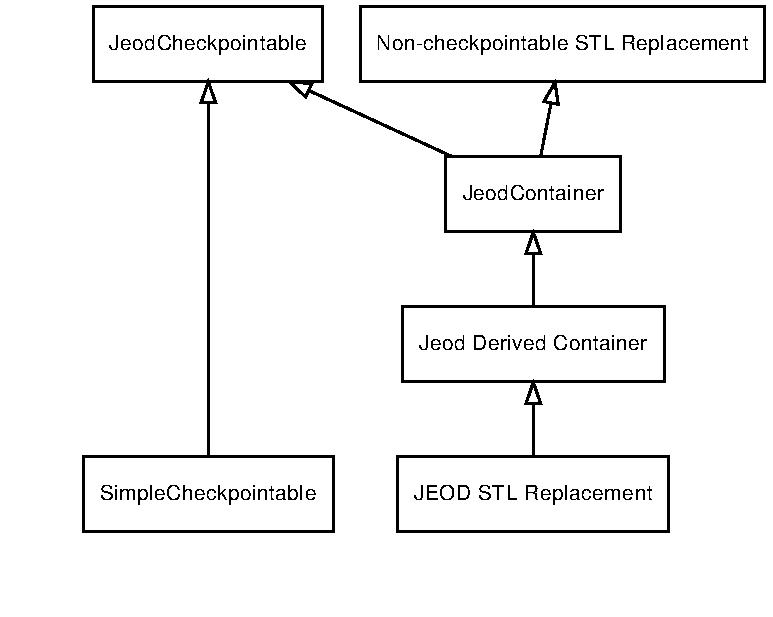
\includegraphics{basics}
\caption{Class Hierarchy (Summary)}
\label{fig:basics}
\end{figure}


Figure \ref{fig:basics} portrays a stylized depiction of the class hierarchy of
the \ModelDesc classes. The left side of the diagram portrays the classes
SimpleCheckpointable and JeodCheckpointable.
JeodCheckpointable is the
base class that specifies in an abstract sense the interfaces needed to
make an object checkpointable. The SimpleCheckpointable implements several
of these behaviors but adds one new pure virtual interface that a derived
class must implement.

On the right side of the diagram, the ``Non-checkpointable STL Replacement''
represents one of the class templates (three provided with this release)
that encapsulate STL container objects. The class template JeodContainer
augments a non-checkpointable STL replacement with a generic set of
checkpoint/restart capabilities.
The JeodContainer does not specify how to translate content to and from the
textual representations used in a JEOD checkpoint file.
This is the responsibility of one of the three ``Jeod Derived Container''
templates. Finally, ``JEOD STL Replacement'' represents one
of the class templates designed as checkpointable replacements for the STL
containers. There are nine such class templates provided with this release.
The remainder of this section expands on the right side of
figure~\ref{fig:basics}.

\subsubsection{Non-Checkpointable STL Replacements}
\begin{figure}[hbtp]
\centering
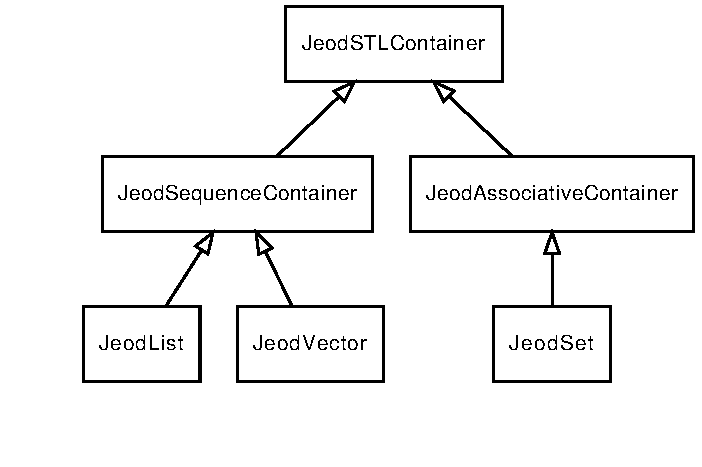
\includegraphics{stl_replacements_generic}
\caption{Non-Checkpointable STL Replacement Classes}
\label{fig:non_checkpointable_stl_replacements}
\end{figure}


Figure \ref{fig:non_checkpointable_stl_replacements} expands upon the
``Non-checkpointable STL Replacement'' node in figure~\ref{fig:basics}.
That node in figure~\ref{fig:basics} represents one of the three nodes at
the bottom of figure~\ref{fig:non_checkpointable_stl_replacements}.

At the top of the diagram, JeodSTLContainer is the base class template for
the non-checkpointable STL replacements. This class encapsulates an STL
container object of the appropriate type and provides types and functions that
are common to all STL containers.
JeodSequenceContainer augments the JeodSTLContainer with methods that are not
common to all STL containers but are common to all STL sequence containers
(std::deque, std::list, and std::vector). 
JeodAssociativeContainer similarly augments the JeodSTLContainer with respect
to STL associative containers (std::map, std::multimap, std::set, and
std::multiset).

At the bottom of the diagram, JeodList, JeodVector, and JeodSet are functionally
near-equivalents to std::list, std::vector, and std::set.
These class templates add functionality unique to std::list, std::vector,
and std::set, as appropriate.
These templates invoke the parent class template in a way that specifies
which STL container template is being replaced.

\subsubsection{Checkpointable STL Replacements}
Figure \ref{fig:stl_replacements_expansion} expands upon the
``JEOD STL Replacement'' node in figure~\ref{fig:basics}.
That node in figure~\ref{fig:basics} represents one of the three nodes at
the bottom of figure~\ref{fig:stl_replacements_expansion}, each of which
in turn represents three specific class template types.
Nine end-user class templates are provided with this release, representing
the set product
\{Object, Pointer, Primitive\} $\times$ \{List,Vector, Set\}.

\begin{figure}[htbp]
\centering
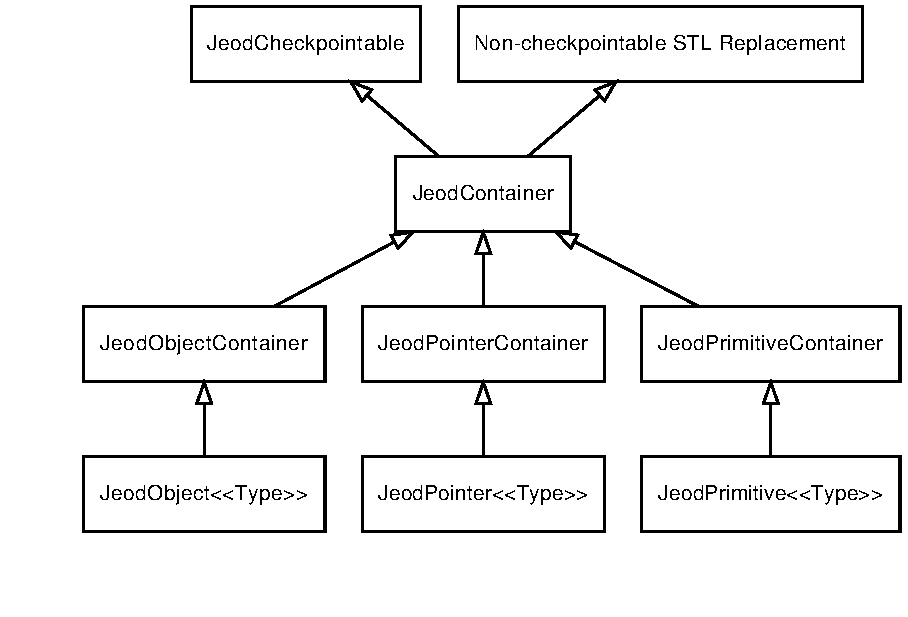
\includegraphics{stl_replacements_expansion}
\caption{Checkpointable STL Replacement Classes (Generic)}
\label{fig:stl_replacements_expansion}
\end{figure}

The class template JeodContainer is the central nexus in
figure~\ref{fig:stl_replacements_expansion}. JeodContainer inherits from
JeodCheckpointable and from a ``Non-checkpointable STL Replacement'',
one of JeodList, JeodVector, or JeodSet.
Exactly which one of the three is specified as a template argument
to JeodContainer. JeodContainer is a mixin class template.
It adds checkpoint/restart capabilities to the functionality of a
non-checkpointable STL replacement container.

JeodContainer implements all but one of the pure virtual methods
declared in JeodCheckpointable and declares one new pure virtual method.
These two unimplemented virtual methods address the problems of translating
an element of a list, vector, or set to a string on checkpoint
and restoring such an element from a string on restart.
The type of data being stored (but not the type of the container) dictates
how these translations to and from a string are performed. Each of the three
template classes JeodObjectContainer, JeodPointerContainer, and
JeodPrimitiveContainer provides implementations of these remaining
virtual methods.

A user could use JeodObjectContainer et al. to specify the type of a
checkpointable STL container replacement. Doing so would be very verbose and
easy to get wrong. As a convenience, JEOD provides nine end-user templates
that represent the set product
\{Object, Pointer, Primitive\} $\times$ \{List,Vector, Set\}.
Using these end-user template typedefs is the recommended technique for
specifying the type of a JEOD STL container replacement object. These
are collectively displayed as the three types at the bottom of
figure~\ref{fig:stl_replacements_expansion}. Figure~\ref{fig:stl_replacements_examples} depicts the inheritance
hierarchy for two of these nine class templates.

\begin{figure}[hbtp]
\centering
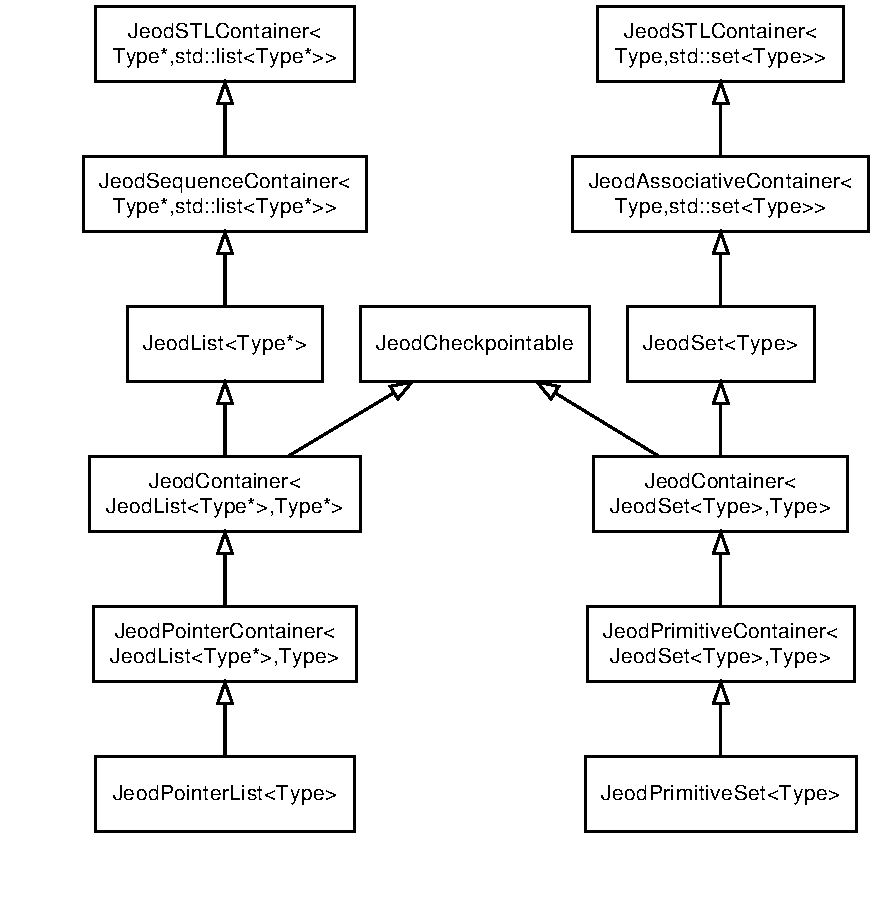
\includegraphics{stl_replacements_examples}
\caption{Checkpointable STL Replacement Classes (Examples)}
\label{fig:stl_replacements_examples}
\end{figure}

\clearpage

\subsection{Class JeodCheckpointable}
\label{sec:spec_JeodCheckpointable}
JeodCheckpointable is the base class for all JEOD checkpointable objects.
As currently implemented, the class contains no member data.
The class defines a number of virtual methods, some pure virtual, others
with an empty default implementation, organized below into five groups.
These groups are:
\begin{itemize}
\item Initialization Method (one method).
\item Checkpoint Control Methods (three methods).
\item Checkpoint Content Methods (four methods).
\item Restart Method (one method).
\item Pre- and Post- Checkpoint and Restart Methods (four methods).
\end{itemize}

\subsubsection{Initialization Methods}
There is one method in this group, initialize\funder{}checkpointable.
\paragraph{initialize\funder{}checkpointable.}
All JeodCheckpointable objects must be registered to make the objects
checkpointable and restartable. The registration machinery calls a
JeodCheckpointable object's initialize\funder{}checkpointable method to signal
that the object has been registered.
The default implementation is to do nothing.

\subsubsection{Checkpoint Control Methods}
Three methods,
start\funder{}checkpoint,
is\funder{}checkpoint\funder{}finished, and
advance\funder{}checkpoint,
control the checkpoint generation process.
The simulation engine interface dumps the contents of a JeodCheckpointable
object via the following loop:
    \begin{verbatim}
    for (checkpointable->start_checkpoint();
         !checkpointable->is_checkpoint_finished();
         checkpointable->advance_checkpoint()) {
       // Record contents at the current checkpoint location, code elided.
    }   
    \end{verbatim}
Each of the methods in this group is pure virtual.

\paragraph{start\_checkpoint.}
The simulation engine calls the start\funder{}checkpoint method to signal the
checkpointable object to prepare for a checkpoint. Some examples:
\begin{itemize}
\item A state machine-based implementation will set some
internal checkpoint state machine to its initial state.
\item An iterator-based implementation will set some
internal checkpoint iterator to the first item to be checkpointed.
\item Other implementations such as the SimpleCheckpointable class will do
nothing at all.
\end{itemize}

\paragraph{is\_checkpoint\_finished.}
The simulation engine calls the is\funder{}checkpoint\funder{}finished method to
determine whether the checkpoint loop should be terminated. This method should
return true when the checkpoint process is complete, false up until that point.
Some examples:
\begin{itemize}
\item A state machine-based implementation will return true when the
internal checkpoint state machine reaches its final state.
\item An iterator-based implementation will return true when the
internal checkpoint iterator reaches the end().
\end{itemize}
The checkpoint loop can be bypassed in its entirety by making the
is\funder{}checkpoint\funder{}finished always return true. This is the approach
taken by the SimpleCheckpointable class.  The advance\funder{}checkpoint,
get\funder{}item\funder{}name, and get\funder{}item\funder{}value methods will
never be called in derived classes that employ this approach. Although never
called, such classes will still need to provide implementations of these three
methods because they are pure virtual.

\paragraph{advance\_checkpoint.}
The simulation engine calls the advamce\funder{}checkpoint method to signal the
checkpointable object to advance itself to the next item to be checkpointed.
Some examples:
\begin{itemize}
\item A state machine-based implementation will advance the
internal checkpoint state machine to the next state.
\item An iterator-based implementation will increment the
internal checkpoint iterator.
\end{itemize}

\subsubsection{Checkpoint Content Methods}
JeodCheckpointable declares four methods that the checkpoint machinery
calls to dump the contents of a checkpointable object.
Each of these methods must return a string.
\paragraph{get\_init\_name and get\_init\_value.}
The checkpoint machinery writes a checkpoint file entry for the
checkpointable object that contains the values returned by these two methods,
but only if the string returned by get\_init\_name is not empty.
This occurs prior to the checkpoint loop described above.
Some examples:
\begin{itemize}
\item get\_init\_name returns ``clear'' for the JEOD STL replacement classes.
The corresponding restart action is to clear the contents of the
object so that the follow-on actions will restore the contents of the
STL object.
\item get\_init\_name returns ``restore'' for the SimpleCheckpointable class.
The corresponding restart action is to call the checkpointable object's
simple\_restore method (which must be implemented by the class that
derives from SimpleCheckpointable.)
\end{itemize}

\paragraph{get\_item\_name and get\_item\_value.}
The checkpoint machinery writes a checkpoint file entry for the
checkpointable object that contains the values returned by these two methods.
These methods are called from within the checkpoint loop described above.

\paragraph{Constraints.}
The following constraints apply to the implementations of these get\_ methods:
\begin{itemize}
\item get\_init\_name must return either the empty string or an
alphanumeric string.
\item get\_item\_name must return a non-empty alphanumeric string.
\item The strings returned by get\_init\_value and get\_item\_value must
not contain characters that force a newline or carriage return.
\end{itemize}
Violating these constraints results in undefined behavior.

Exception: The constraint on get\_item\_name does not apply if that method is
guaranteed to never be called, \emph{i.e.} the is\_checkpoint\_finished method
always returns true. The get\_item\_name method must still be defined to make
the class in question viable, but the implementation can be to return the
empty string.

\subsubsection{Restart Methods}
There is one method in this group, perform\_restore\_action.
\paragraph{perform\_restore\_action.}
The restart machinery calls this method for every entry in the checkpoint
file that pertains to the JeodCheckpointable object. This method takes
two arguments, both of them const references to STL strings. The first argument,
action\_name, is a string returned by the get\_init\_name or get\_item\_name
method. The second argument, action\_value, is the corresponding value.
A typical implementation will be in the form of an if/else if/else set of
statements keyed on the action\_name. 

\subsubsection{Pre and Post Checkpoint and Restart Methods}
JeodCheckpointable defines four methods that are called before and
after the checkpoint or restart proper. The default implementation for
each does nothing.
\paragraph{pre\_checkpoint.}
This method is called before any resources are checkpointed.
Data allocated by JEOD\_ALLOC in a pre\_checkpoint method will be checkpointed.
The JeodObjectContainer uses this capability to create a checkpointable
copy of the STL container. JeodCheckpointable extenders may wish to
emulate this behavior.
\paragraph{post\_checkpoint.}
This method is called after checkpointing is complete.
The array allocated by the JeodObjectContainer pre\_checkpoint method
is used only for checkpoint and restart.
The JeodObjectContainer post\_checkpoint method frees this array.
\paragraph{pre\_restart.}
This method is called before any resources are restored.
One envisioned use of this method is in a class that needs to free resources
prior to restoring them to avoid leaks. Note: Allocating resources in this
method is not recommended as doing so most likely will be a leak.
\paragraph{post\_restart.}
This method is called after restart proper.
One envisioned use of this method is in a class that needs to restore a
resource that crosses class boundaries.

\subsection{Class SimpleCheckpointable}
The SimpleCheckpointable class provides a simple checkpoint/restart interface
by which an object can complete the restart process. JEOD uses this class to
restore the DE4xx ephemeris file stream and to restore the function pointers
in a JEOD integrator.
The class derives from JeodCheckpointable and implements all of the pure virtual
methods declared in JeodCheckpointable.

The class SimpleCheckpointable declares one pure virtual interface,
simple\funder{}restore. Classes that
derive from SimpleCheckpointable must provide an implementation of this
method to make the derived class complete. Derived classes should not
override the methods declared in JeodCheckpointable and implemented in
JeodCheckpointable. Derived classes can override the pre\_ and post\_checkpoint
and the pre\_ and post\_restart methods.


\subsection{Non-Checkpointable STL Replacement Class Templates}
\label{sec:spec_noncheckpointable_stl_replacements}
JEOD provides non-checkpointable STL replacement class templates for
std::list (JeodList), std::set (JeodSet), and std::vector (JeodVector).
These class templates, per self-imposed requirements and by design,
are near-equivalents of the targeted STL class templates. The places where
the JEOD class templates differ from their STL counterparts as specified
in the 2003 \Cplusplus Standard (ISO/IEC 14882:2003 \cite{cpp2003}) are:
\begin{itemize}
\item The destructors for the JEOD class templates, unlike their STL
counterparts, are virtual. That STL containers have non-virtual
destructors means a class cannot safely derive from an STL container.
This is the key factor that drove the development of
this part of the model.
\item The constructors for the JEOD class templates, unlike their STL
counterparts, do not take optional arguments. Users of the JEOD container
class templates cannot provide an alternate Allocator class or
an alternate Compare object.
\item The standard specifies a number of constructors for the STL containers.
The JEOD implementation provides only two of these: Default and copy.
\item The constructors are protected rather than public. The non-checkpointable
STL replacement class templates are not designed for use by the end-user.
\item The swap function is protected rather than public. The checkpointable
STL replacement class templates later exports this functionality in the form of
the swap\_contents function. This function swaps the STL content of two
objects but leaves the content related to checkpoint/restart untouched.
(This in turn means swap\_contents cannot be called ``swap'' per the
standard committee's concept of being ``swappable''.)
\item JeodSet implements the non-const iterator as a const\_iterator and
implements find, lower\_bound, upper\_bound, and equal\_range as specified
in table 69 of the 2003 \Cplusplus Standard rather than as specified in
section 23.3.3 of the standard. (These implementations are consistent with the
GNU implementations and with the recommendations of the
\Cplusplus Standards Committee.)
\end{itemize}

To reduce the amount of replicated code, the JEOD implementations of these
end-user class templates inherit from JeodSequenceContainer (JeodList and
JeodVector) or JeodAssociativeContainer (JeodSet), both of which in turn
inherit from JeodSTLContainer.
The JeodSTLContainer class template defines items common to all STL
containers. The class templates JeodSequenceContainer and
JeodAssociativeContainer add items
common to all sequence containers and associative containers. The end-user
classes specify non-common content only.

In addition to defining items common to all STL containers, a JeodSTLContainer
also contains a data member that is an STL container of the type being
replaced. One way to look at the JEOD STL container replacement class templates
is that they aren't truly STL container replacements. They are instead STL
container encapsulators that transparently provide the functionality of
the the encapsulated objects.

\subsection{Checkpointable STL Replacement Class Templates}
The ultimate goal of the STL container replacement aspect of this model is
to make the non-checkpointable class templates described in
section~\ref{sec:spec_noncheckpointable_stl_replacements} checkpointable.
The starting point for this effort is the class template JeodContainer.
JeodContainer inherits from JeodCheckpointable and from one of the
non-checkpointable STL container replacement class templates, specified as one
of the template arguments to JeodContainer.

JeodContainer makes a non-checkpointable container object checkpointable
without needing to know specifics of the type container that is being
encapsulated. It accomplishes this by using three features common to all STL
containers, including those not yet encapsulated by this model:
\begin{itemize}
\item Iterators that can be used to walk over the
contents of the container object from beginning to end,
\item A clear() method that empties the container object, and
\item An insert(iterator, value) method that can be
used to add some value to the end of the container object.
\end{itemize}
By taking advantage of these common features, the JeodContainer by itself
comes very close to adding checkpoint/restart capabilities to a container.
The class defines all but one of the functions declared as pure virtual
in JeodCheckpointable.

What JeodContainer cannot do is translate the value of a container element to a
string or recreate the element value given the string representation.
JeodContainer does not implement the get\funder{}item\funder{}value method
declared as pure virtual in JeodCheckpointable and declares
perform\funder{}insert\funder{}action as a new pure
virtual method. The details of how containers of objects, pointers, and
primitives are checkpointed and restored are handled by the three class
templates JeodObjectContainer, JeodPointerContainer, and JeodPrimitiveContainer,
each of which derives from JeodContainer and each of which implements
those two remaining pure virtual methods in a different manner.

The class template JeodObjectContainer targets containers of objects.
It achieves checkpoint/restart by creating a C-style array copy of the
container. The array and its contents are checkpointed and restored using
the simulation engine's native checkpoint/restart capabilities. The
container is restored by copying the contents of the restored array back
into the container.

The class template JeodObjectContainer targets containers of pointers. It's
get\funder{}item\funder{}value and perform\funder{}insert\funder{}action methods
use the \SIMINTERFACE\ to translate an address to and from a
string representation.

The class template JeodPrimitiveContainer targets containers of items
that can be translated to and from a string using the insertion and
extraction operators. The class uses the template class JeodPrimitiveSerializer
to assist in this serialization and deserialization.

A user could use JeodObjectContainer et al. to specify the type of a
checkpointable STL container replacement. As mentioned above, this is
verbose and error prone, and thus is not the recommended usage.
JEOD provides nine end-user templates that represent the set product
\{Object, Pointer, Primitive\} $\times$ \{List,Vector, Set\}.

\clearpage
\boilerplateinventory
